\documentclass[../../lecture_notes.tex]{subfiles}
\begin{document}


Take the ORNL Cray Cluster Star

\begin{minipage}{0.5\linewidth}
\begin{itemize}
	\item Storage: 1 EB ($10^18$ bytes $\rightarrow$ 1 million TB)
	\item Speed: 10 TB/s output
	\item Size: 40 cabinets with 19 inch racks
	\item Cost: \$50 million
	\item Utilizes flash and disk
	\item 2 systems: 
		\begin{itemize}
			\item Lustre for distributed 
			\item ZFS for local
		\end{itemize}
\end{itemize}
\end{minipage}%
\hfill
\begin{minipage}{0.5\linewidth}
\begin{center}
\begin{tabular} { r | c | c | }
	\multicolumn{1}{c}{} & \multicolumn{1}{c}{Flash} & \multicolumn{1}{c}{Disk} \\
	\cline{2-3}
	Cost & \$110/TB & \$14/TB \\
	\cline{2-3}
	Reliability & & \checkmark \\
	\cline{2-3}
	Durability & & \checkmark \\
	\cline{2-3}
	Speed & \checkmark & \\
	\cline{2-3}
\end{tabular}
\end{center}
\end{minipage}


How do we judge performance?
\begin{enumerate}[ label=(\alph*), nosep]
	\item throughput $\coloneqq$ total requests or bytes per second (read is advertised, since it’s fast)
	\item latency $\coloneqq$ delay between request and response
	\item utilization $\coloneqq$ fraction of capacity doing useful work
\end{enumerate}

But (a) and (b) are competing values!

What strategies do we have?

\begin{minipage}{0.5\linewidth}
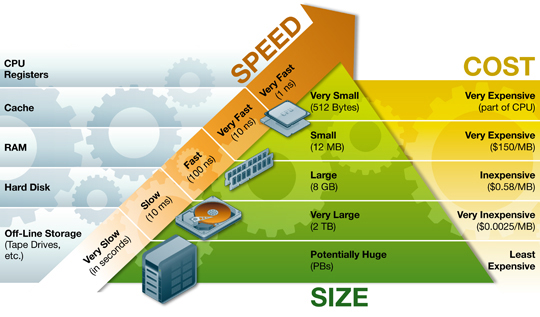
\includegraphics[width=0.9\linewidth]{tradeoff_pyramid}
\end{minipage}%
\begin{minipage}{0.5\linewidth}
We exploit locality of reference by caching data we expect to need into higher memory:
\begin{itemize}[nosep]
	\item spacial locality $\coloneqq$ accessing address $i$ means accessing address $i \pm 1$ is likely
	\item temporal locality $\coloneqq$ accessing address $i$ means accessing i again is likely
\end{itemize}
\end{minipage}

The file system takes advantage of this locality in 3 main ways:
\begin{itemize}
\item Prefetching $\coloneqq$ the OS caches memory it expects to need ahead of time
\item Batching $\coloneqq$ the OS reads all around a piece of data on read (includes prefetching)
\item Dallying $\coloneqq$ the OS caches writes with the hopes that it can perform adjacent writes
\end{itemize}

But what if we need the data to be written NOW?
\begin{lstlisting}
sync();
// flush all buffers to permanent storage
// performed system wide, so it is often a waste of effort
fsync(int fd);
// flush all buffers for a given file descriptor and wait for completion
fdatasync(int fd);
// flush all data buffers for a given file descriptor and wait for completion
// fast, since metadata is the slow part (it is stored in memory)
\end{lstlisting}


The IBM General Parallel File System uses a few other tricks for optimization:
\begin{itemize}
\item Striping
\item Distributed Metadata $\coloneqq$ Copies of file metadata exist to alleviate IO bottleneck
\item Distributed Locking $\coloneqq$ Systems allow users to lock sections of file, and not the whole file
\item Efficient Directory Indexing $\coloneqq$ GPFS uses a fancier data structure to represent files.
\item File System Stays Live During Maintenance
\end{itemize}

\subsection{File Systems}
$\coloneqq$ a data structure for primary and secondary storage with support for searching.

\subsubsection{Very Simple File System (RT-11)}

\begin{center}
\begin{tikzpicture}

% ROW 1
\node[rectangle, draw, minimum width=2cm, minimum height=1cm] (11) {TOC};
\node[rectangle, draw, minimum width=2cm, minimum height=1cm, right=0cm of 11] (12) {File 1};
\node[rectangle, fill=gray, draw, minimum width=1cm, minimum height=1cm, right=0cm of 12] (13) {};
\node[rectangle, draw, minimum width=2cm, minimum height=1cm, right=0cm of 13] (14) {File 2};
\node[rectangle, fill=gray, draw, minimum width=1cm, minimum height=1cm, right=0cm of 14] (15) {};
\node[rectangle, draw, minimum width=2cm, minimum height=1cm, right=0cm of 15] (16) {File 3};
\node[rectangle, draw, minimum width=2cm, minimum height=1cm, right=0cm of 16] (17) {File 4};
\node[rectangle, fill=gray, draw, minimum width=3cm, minimum height=1cm, right=0cm of 17] (15) {};

% ROW 2
\node[rectangle, draw, minimum width=2cm, minimum height=1cm, below= of 11] (21) {\scriptsize File 1 Entry};
\node[rectangle, draw, minimum width=2cm, minimum height=1cm, right=0cm of 21] (22) {\scriptsize File 2 Entry};
\node[rectangle, draw, minimum width=2cm, minimum height=1cm, right=0cm of 22] (23) {\scriptsize File 2 Entry};
\node[rectangle, draw, minimum width=1cm, minimum height=1cm, right=0cm of 23] (24) {\scriptsize $\cdots$};
\node[rectangle, fill=gray, draw, minimum width=3cm, minimum height=1cm, right=0cm of 24] (25) {};

% ROW 3
\node[rectangle, draw, minimum width=2cm, minimum height=1cm, below= of 21] (31) {\scriptsize File Name};
\node[rectangle, draw, minimum width=2cm, minimum height=1cm, right=0cm of 31] (32) {\scriptsize Start Location};
\node[rectangle, draw, minimum width=2cm, minimum height=1cm, right=0cm of 32] (33) {\scriptsize File Size};

% ARROWS
\draw[-Latex] (11.south west) -- (21.north west); \draw[-Latex] (11.south east) -- (25.north);
\draw[-Latex] (21.south west) -- (31.north west); \draw[-Latex] (21.south east) -- (33.north east);

\node[rectangle, fill=gray, draw, minimum width=1cm, minimum height=1cm, right=2cm of 25, 
	label=east:{\scriptsize Unused Space}] {};
\end{tikzpicture}
\end{center}

RULES:
	\begin{itemize}
		\item 2mb of memory broken into 512 byte sectors
		\item files start on sector boundaries
		\item files are continuous (like in RT-11)
		\item sectors will only be partially used
		\item first 10 sectors form a table of contents
		\item file size is statically decided on creation
		\item first byte indicates if the directory is full
		\item files can only span a single region of free space
	\end{itemize}
PROS:
	\begin{itemize}
		\item predictable
		\item easy truncation
		\item good sequential access
	\end{itemize}
CONS
	\begin{itemize}
		\item file number limit ($2^6$)
		\item difficult to grow files
		\item only one directory — no user ones
		\item no file permissions
		fragmentation
			\begin{itemize}
				\item internal $\coloneqq$ wasted data within allocated space
				\item external $\coloneqq$ scattered and therefore unusable free space
			\end{itemize}
	\end{itemize}


\subsubsection{FAT File System}

The VSFS was the primary file system until Bill Gates came along in the 70s and created…

\begin{center}
\begin{tikzpicture}
\node[rectangle, draw, minimum width=0.5cm, minimum height=1cm, align=center] (11) {};
\node[left=of 11, anchor=center, align=center] (BB){Boot\\Block}; \draw (BB) -- (11);
\node[rectangle, draw, minimum width=2cm, minimum height=1cm, right=0cm of 11, align=center] (12) 
	{Super\\Block};
\node[rectangle, draw, minimum width=3cm, minimum height=1cm, right=0cm of 12] (13) {FAT};
\node[rectangle, draw, minimum width=1cm, minimum height=1cm, right=0cm of 13] (14) {1};
\node[rectangle, draw, minimum width=1cm, minimum height=1cm, right=0cm of 14] (15) {2};
\node[rectangle, fill=gray, draw, minimum width=1cm, minimum height=1cm, right=0cm of 15] (16) {3};
\node[rectangle, draw, minimum width=1cm, minimum height=1cm, right=0cm of 16] (17) {4};
\node[rectangle, fill=gray, draw, minimum width=4cm, minimum height=1cm, right=0cm of 17] (18) {$\cdots$};
% FAT
\node[below=of 13, rectangle, draw, minimum width=1cm, minimum height=0.5cm] (23) {-1}; 
\node[right=0cm of 23, rectangle, draw, minimum width=1cm, minimum height=0.5cm] (24) {N}; 
\node[right=0cm of 24, rectangle, draw, minimum width=1cm, minimum height=0.5cm] (25) {$\cdots$}; 
\node[right=0cm of 25, rectangle, draw, minimum width=1cm, minimum height=0.5cm] (26) {0}; 
\node[left=0cm of 23, rectangle, draw, minimum width=1cm, minimum height=0.5cm] (22) {27}; 
\node[left=0cm of 22, rectangle, draw, minimum width=1cm, minimum height=0.5cm] (21) {2573}; 
\node[left=0cm of 21, rectangle, draw, minimum width=1cm, minimum height=0.5cm] (20) {916}; 
\draw[dashed] (13.south west) -- (20.north west); \draw[dashed] (13.south east) -- (26.north east);
\draw[Latex-Latex] (23.north) -- (16.south);
\end{tikzpicture}
\end{center}


The goal: turn files into linked lists of blocks to avoid external fragmentation.

RULES:
	\begin{enumerate}[nosep]
		\item Blocks contain discrete size blocks of file data
		\item Boot block contains setup code
		\item A \term{super block} is fixed size and contains the file system's
			\begin{itemize}
				\item Size
				\item Version number
				\item Number of blocks in use
				\item Root directory block number
			\end{itemize}
		\item FAT contains address of the block which comes next in the file
			\begin{itemize}
				\item -1 $\iff$ Free block in file system
				\item 0 $\iff$ EOF (last block in current file)
				\item N $\iff$ Next block in this file is N
			\end{itemize}
		\item Directories form a tree rooted at the root directory
		\item Directories contain data blocks just like files, but the form is different, as follows:
	\end{enumerate}
\begin{center}
\begin{tikzpicture}
% Blocks
\node[rectangle, draw, minimum width=2cm, minimum height=1cm, 
	label=above:{\scriptsize 8}] (11) {\scriptsize File Name};
\node[rectangle, draw, minimum width=0.75cm, minimum height=1cm, right=0cm of 11, 
	label=above:{\scriptsize 3}] (12) {};
\node[rectangle, draw, minimum width=0.25cm, minimum height=1cm, right=0cm of 12, 
	label=above:{\scriptsize 1}] (13) {};
\node[rectangle, fill=gray, draw, minimum width=2.5cm, minimum height=1cm, right=0cm of 13, 
	label=above:{\scriptsize 10}] (14) {}; 
\node[rectangle, draw, minimum width=0.5cm, minimum height=1cm, right=0cm of 14, 
	label=above:{\scriptsize 2}] (15) {};
\node[rectangle, draw, minimum width=0.5cm, minimum height=1cm, right=0cm of 15, 
	label=above:{\scriptsize 2}] (16) {};
\node[rectangle, draw, minimum width=0.5cm, minimum height=1cm, right=0cm of 16, 
	label=above:{\scriptsize 2}] (17) {};
\node[rectangle, draw, minimum width=1cm, minimum height=1cm, right=0cm of 17, 
	label=above:{\scriptsize 4}] (18) {\scriptsize Size};
% Labels
\node[below=of 12, anchor=center, rotate=270] (EXT) {\scriptsize Extension}; \draw (12) -- (EXT);
\node[below=of 13, anchor=center, rotate=270] (ATT) {\scriptsize Attributes}; \draw (13) -- (ATT);
\node[below=of 14, anchor=center, rotate=270] (RES) {\scriptsize Reserved}; \draw (14) -- (RES);
\node[below=of 15, anchor=center, rotate=270] (TIME) {\scriptsize Time}; \draw (15) -- (TIME);
\node[below=of 16, anchor=center, rotate=270] (DATE) {\scriptsize Date}; \draw (16) -- (DATE);
\node[below=of 17, anchor=center, rotate=270] (BLOCKNO) {\scriptsize First Block \#}; \draw (17) -- (BLOCKNO);
\end{tikzpicture}
\end{center}

PROS:
	\begin{itemize}
		\item no external fragmentation
		\item no preallocation
		\item large file count limit
	\end{itemize}
CONS:
	\begin{itemize}
		\item internal fragmentation is not fixed
		\item can be addressed by periodic defragmentation of files; this is both costly and risky
		\item moving a file to another directory can lose both copies, so this is forbidden
		\item no random access --- we would need to walk through the whole list to find a byte offset
	\end{itemize}
Random access was important to Unix, so Linux made this easy


\end{document}